\documentclass[aspectratio=169]{beamer}

\usetheme{Madrid}
\usecolortheme{whale}
\setbeamertemplate{navigation symbols}{}
\setbeamercovered{transparent}

\usepackage[T1]{fontenc}
\usepackage[utf8]{inputenc}
\usepackage{amsmath,amssymb}
\usepackage{booktabs}
\usepackage{graphicx}
\usepackage{xcolor}
\usepackage{listings}
\usepackage{tikz}

\graphicspath{{figures/}}

% Shorthands, same notation as the written report.
\newcommand{\R}{\mathbb{R}}
\newcommand{\muhat}{\hat{\mu}}
\newcommand{\Sig}{\Sigma}
\newcommand{\Ssqrt}{\Sigma^{1/2}}
\newcommand{\one}{\mathbf{1}}
\newcommand{\norm}[1]{\left\lVert #1 \right\rVert}
\newcommand{\prox}{\operatorname{prox}}
\newcommand{\softt}{\mathcal{S}}

\definecolor{codegray}{gray}{0.4}
\lstset{
  basicstyle=\ttfamily\scriptsize,
  commentstyle=\color{codegray}\itshape,
  numbers=none, breaklines=true, breakatwhitespace=false,
  showstringspaces=false, frame=single, rulecolor=\color{codegray},
  tabsize=4,
}

\newcommand{\good}[1]{\textcolor{green!45!black}{\textbf{#1}}}
\newcommand{\bad}[1]{\textcolor{red!60!black}{\textbf{#1}}}

\title[Sparse + Robust Portfolio Opt.]{Sparse and Robust Mean--Variance\\Portfolio Optimization on VN100}
\subtitle{A hand-written proximal-subgradient method, cross-verified against an interior-point solver}
\author[N.\,T.\ Binh]{Nguyen To Binh \\ \small Student ID: 1010051 --- Individual project}
\institute[]{TODO: Course name and code \\ TODO: Instructor name}
\date[\today]{\today}

\begin{document}

\begin{frame}
  \titlepage
\end{frame}

\begin{frame}{Outline}
  \tableofcontents
\end{frame}

% ============================================================
\section{Motivation}
% ============================================================
\AtBeginSection[]{
  \begin{frame}{Outline}
    \tableofcontents[currentsection]
  \end{frame}
}

\begin{frame}{The problem, in plain words}
  An investor has \textbf{1 unit of capital} and must split it across the
  \textbf{98 stocks} of the VN100 basket, using 4 years of daily prices.

  \vspace{0.3cm}
  \textbf{Plain mean--variance (Markowitz) is not enough:}
  \begin{enumerate}
    \item<2-> \textbf{Estimates are noisy.} A sample mean return is a bad estimator over a short
          window --- an optimizer tuned to it is tuned to noise.
    \item<3-> \textbf{Holding 98 stocks is expensive.} Every position costs money to open,
          monitor, and close.
    \item<4-> \textbf{Risk still matters.} Variance of the realized return is a genuine concern.
  \end{enumerate}

  \vspace{0.3cm}
  \onslide<5->{\centering \textit{Goal: one model, one solver, that balances all three.}}
\end{frame}

\begin{frame}{Four objectives $\to$ four terms}
  \[
    \min_{w \in \R^{98}} \quad
      \underbrace{-\muhat^\top w}_{\text{return}}
      \;+\; \underbrace{\kappa \norm{\Ssqrt w}_2}_{\text{robustness}}
      \;+\; \underbrace{\gamma\, w^\top \Sig w}_{\text{variance}}
      \;+\; \underbrace{\lambda \norm{w}_1}_{\text{sparsity}}
    \quad \text{s.t.} \quad \one^\top w = 1
  \]
  \vspace{0.2cm}
  \begin{table}
  \small
  \begin{tabular}{@{}ll@{}}
  \toprule
  \textbf{Term} & \textbf{Role} \\
  \midrule
  $-\muhat^\top w$ & maximize expected return \\
  $\kappa \norm{\Ssqrt w}_2$ & worst case if $\muhat$ is wrong (derived, not assumed --- next section) \\
  $\gamma\, w^\top \Sig w$ & classical Markowitz variance penalty \\
  $\lambda \norm{w}_1$ & convex surrogate for \# holdings; also caps gross leverage \\
  \bottomrule
  \end{tabular}
  \end{table}
  \textbf{No $w \ge 0$}: short selling is allowed --- a deliberate design choice.
\end{frame}

% ============================================================
\section{The model}
% ============================================================

\begin{frame}{Decision variable and constants}
  \textbf{Decision variable:} $w \in \R^{98}$ --- fraction of capital in each stock
  ($w_i < 0$ = short).

  \vspace{0.3cm}
  \textbf{Constants} (estimated once, then fixed):
  \begin{itemize}
    \item $\muhat \in \R^{98}$ --- sample mean daily return
    \item $\Sig \in \mathbb{S}^{98}_+$ --- sample covariance
    \item $\Ssqrt$ --- symmetric PSD square root, $\Ssqrt\Ssqrt = \Sig$
  \end{itemize}

  \vspace{0.3cm}
  \textbf{Hyperparameters} $\kappa,\gamma,\lambda \ge 0$: \emph{not} decision variables ---
  chosen by us (\S~Results) or by validation (backtest).
\end{frame}

\begin{frame}{Type of problem}
  \textbf{Convex.} Every term is convex (affine, norm, PSD quadratic, norm); feasible set is
  affine $\Rightarrow$ \textbf{every local optimum is global, and unique in value.}

  \vspace{0.2cm}
  \textbf{Second-order-cone representable}: an epigraph reformulation turns the two norms into
  SOC constraints and the quadratic into a rotated SOC $\Rightarrow$ solvable by a generic conic
  solver (used later as an independent check).

  \vspace{0.2cm}
  \textbf{Nondifferentiable.} $\kappa\norm{\Ssqrt w}_2$ breaks at $\Ssqrt w = 0$;
  $\lambda\norm{w}_1$ breaks at every zero coordinate --- exactly where the sparse solution
  lives. \good{Plain gradient descent cannot be used.}

  \vspace{0.3cm}
  \begin{center}
  \Large $\Rightarrow$ we need a \textbf{proximal-subgradient} method.
  \end{center}
\end{frame}

% ============================================================
\section{Worked example, step by step}
% ============================================================

\begin{frame}{A toy example: 3 assets (illustrative numbers, not real data)}
  To make every formula concrete, take $N=3$ fictitious assets A, B, C.
  \[
    \muhat = \begin{pmatrix}0.08\\0.05\\0.02\end{pmatrix}
    \qquad
    \Sig = \begin{pmatrix}
      0.10 & 0.02 & 0.01\\
      0.02 & 0.08 & 0.03\\
      0.01 & 0.03 & 0.05
    \end{pmatrix}
  \]
  Eigendecomposing $\Sig$ (all eigenvalues $>0$) gives
  \[
    \Ssqrt \approx \begin{pmatrix}
      0.314 & 0.032 & 0.015\\
      0.032 & 0.274 & 0.060\\
      0.015 & 0.060 & 0.215
    \end{pmatrix}, \qquad \norm{\Ssqrt\Ssqrt-\Sig} \approx 0.
  \]
  Take $\kappa=1,\ \gamma=5,\ \lambda=0.05$, and a starting point
  $w_0 = \left(\tfrac13,\tfrac13,\tfrac13\right)$.
\end{frame}

\begin{frame}{Step 1 --- evaluate the objective at $w_0$}
  \begin{align*}
    -\muhat^\top w_0 &= -0.0500 \\
    w_0^\top \Sig w_0 &= 0.0389 \\
    \norm{\Ssqrt w_0}_2 &= 0.1972 \\
    \norm{w_0}_1 &= 1.0000
  \end{align*}
  \[
    f(w_0) = -0.0500 + \underbrace{1}_{\kappa}\!\cdot 0.1972
      + \underbrace{5}_{\gamma}\!\cdot 0.0389 + \underbrace{0.05}_{\lambda}\!\cdot 1.0000
      = \good{0.3916}
  \]
  This is the number the algorithm will try to \textbf{decrease}.
\end{frame}

\begin{frame}{Step 2 --- what does ``robust'' concretely buy us?}
  Worst-case mean over the uncertainty ellipsoid
  $\mathcal{U}=\{\muhat+\Ssqrt u : \norm{u}_2\le\kappa\}$ is attained at
  $u^\star = -\kappa\,\Ssqrt w_0/\norm{\Ssqrt w_0}_2$:
  \[
    u^\star \approx (-0.612,\,-0.621,\,-0.491), \qquad \norm{u^\star}_2 = 1 = \kappa
  \]
  \[
    \mu_{\text{worst}} = \muhat + \Ssqrt u^\star \approx (-0.140,\,-0.170,\,-0.132)
  \]
  \textbf{Check:} $-\mu_{\text{worst}}^\top w_0 = 0.1472$, and indeed
  \[
    -\muhat^\top w_0 + \kappa\norm{\Ssqrt w_0}_2 = -0.0500 + 0.1972 = \good{0.1472} \checkmark
  \]
  The robust term is not a heuristic --- it \emph{is} this worst case, exactly.
\end{frame}

\begin{frame}{Step 3 --- the subgradient at $w_0$}
  \[
    v_0 = -\muhat + 2\gamma\,\Sig w_0 + \kappa\,\frac{\Sig w_0}{\norm{\Ssqrt w_0}_2}
  \]
  \begin{align*}
    \Sig w_0 &\approx (0.0433,\ 0.0433,\ 0.0300) \\
    \text{robust part } \kappa\,\Sig w_0/\norm{\Ssqrt w_0}_2 &\approx (0.2197,\ 0.2197,\ 0.1521) \\
    v_0 &\approx (0.5731,\ 0.6031,\ 0.4321)
  \end{align*}
  \bad{Common mistake:} the numerator is $\Sig w_0$ (full covariance), \emph{not}
  $\Ssqrt w_0$ --- easy to write wrong, and the wrong version still runs, just converges to
  the wrong point.
\end{frame}

\begin{frame}{Step 4 --- take a step}
  \[
    z = w_0 - \alpha\, v_0
  \]
  Using a small illustrative step $\alpha=0.3$ (the real solver uses a schedule
  $\alpha_k=\alpha_0/\sqrt{k+1}$ tuned for the 98-asset scale):
  \[
    z \approx (0.1614,\ 0.1524,\ 0.2037), \qquad \sum_i z_i = 0.5175
  \]
  Notice $z$ does \emph{not} sum to 1 --- the step alone breaks the budget constraint.
  \vspace{0.2cm}
  \begin{center}
  \Large $\Rightarrow$ we need to project it back, \emph{while also} soft-thresholding for
  sparsity.
  \end{center}
\end{frame}

\begin{frame}{Step 5 --- the joint prox: soft-threshold \emph{and} rebudget at once}
  Solve $w_1 = \arg\min_w \tfrac12\norm{w-z}_2^2 + t\norm{w}_1$ s.t.\ $\one^\top w=1$,
  with $t=\alpha\lambda = 0.3\times0.05 = 0.015$.

  \textbf{Closed form:} $w_i(\nu) = \softt_t(z_i+\nu)$ (soft threshold); find $\nu$ by
  \textbf{bisection} on $h(\nu)=\sum_i \softt_t(z_i+\nu)-1$.

  \small
  \begin{table}
  \begin{tabular}{@{}ccccc@{}}
  \toprule
  iter & lo & hi & $\nu_{\text{mid}}$ & $h(\nu_{\text{mid}})$ \\
  \midrule
  1 & $-1.000$ & $1.000$ & $0.000$  & $-0.527$ \\
  2 & $0.000$  & $1.000$ & $0.500$  & $+0.973$ \\
  3 & $0.000$  & $0.500$ & $0.250$  & $+0.223$ \\
  4 & $0.000$  & $0.250$ & $0.125$  & $-0.152$ \\
  5 & $0.125$  & $0.250$ & $0.188$  & $+0.035$ \\
  \multicolumn{5}{c}{$\vdots$ (converges after $\sim$40 iters, tol.\ $10^{-12}$)} \\
  \bottomrule
  \end{tabular}
  \end{table}
  \[
    \nu^\star \approx 0.1758 \ \Rightarrow\ w_1 \approx (0.3222,\ 0.3132,\ 0.3645), \quad
    \sum_i w_{1,i} = \good{1.0000}
  \]
\end{frame}

\begin{frame}{Step 6 --- where do the \emph{exact} zeros come from?}
  Same operator, a case where the threshold $t$ is large enough to zero a coordinate.
  Take $z=(0.55,\ 0.20,\ -0.10,\ 0.35)$, $t=0.15$:
  \small
  \begin{table}
  \begin{tabular}{@{}ccccc@{}}
  \toprule
  iter & lo & hi & $\nu_{\text{mid}}$ & $h(\nu_{\text{mid}})$ \\
  \midrule
  1 & $-1.000$ & $1.000$ & $0.000$   & $-0.350$ \\
  2 & $0.000$  & $1.000$ & $0.500$   & $+1.400$ \\
  3 & $0.000$  & $0.500$ & $0.250$   & $+0.400$ \\
  4 & $0.000$  & $0.250$ & $0.125$   & $+0.025$ \\
  5 & $0.000$  & $0.125$ & $0.0625$  & $-0.163$ \\
  \bottomrule
  \end{tabular}
  \end{table}
  Converges to $\nu^\star = \tfrac{7}{60}\approx0.1167$:
  \[
    w^\star \approx (0.5167,\ 0.1667,\ \good{0.0000},\ 0.3167), \qquad \sum_i w^\star_i = 1
  \]
  Coordinate 3 satisfies $|z_3+\nu^\star| = 0.0167 \le t = 0.15$ $\Rightarrow$
  \good{driven to exactly zero} --- not a small number, a true zero.
\end{frame}

\begin{frame}{Recap: one full iteration}
  \begin{enumerate}
    \item Compute the subgradient $v_k$ (Step 3).
    \item Take a descent step: $z_k = w_k - \alpha_k v_k$ (Step 4).
    \item Solve the joint prox by bisection $\Rightarrow$ $w_{k+1}$: feasible \emph{and}
          sparse, simultaneously (Steps 5--6).
    \item Repeat until the (best) objective stops improving.
  \end{enumerate}
  \vspace{0.4cm}
  \begin{center}
  On the real 98-asset problem this takes \good{a few hundred to a few thousand}
  iterations --- shown next.
  \end{center}
\end{frame}

% ============================================================
\section{Algorithm and implementation}
% ============================================================

\begin{frame}[fragile]{The full algorithm}
\begin{lstlisting}[basicstyle=\ttfamily\tiny]
w_0 <- (1/N)*1;  best_obj <- +inf;  stall <- 0
for k = 0, 1, 2, ...:
    r <- ||Sigma^(1/2) w_k||_2
    s <- (Sigma w_k)/r  if r > eps  else  0        # robust subgradient
    v <- -mu_hat + 2*gamma*(Sigma w_k) + kappa*s
    alpha <- alpha_0 / sqrt(k+1)
    z <- w_k - alpha*v
    w_{k+1} <- JointProx(z, t = alpha*lambda)      # bisection, as above
    if objective(w_{k+1}) < best_obj:
        best_obj <- objective(w_{k+1});  best_w <- w_{k+1}
    stop when best_obj has not improved for 100 iterations
return best_w
\end{lstlisting}
  \textbf{Best-iterate, not last-iterate:} a subgradient method is not monotone --- the solver
  tracks and returns the best $w$ seen, not the final one.
\end{frame}

\begin{frame}{Implementation choices}
  \begin{itemize}
    \item \textbf{Pure NumPy.} No \texttt{cvxpy} / \texttt{scipy.optimize} / \texttt{sklearn}
          in the solver --- only in the independent verifier.
    \item $\Ssqrt$ via \textbf{eigendecomposition}, not Cholesky: the sample $\Sig$
          ($N{=}98$, $T{=}965$) is only PSD, with a few numerically negative eigenvalues ---
          clip to 0 before taking the square root.
    \item Reconstruction check: $\norm{\Ssqrt\Ssqrt-\Sig}_F/\norm{\Sig}_F \approx
          \textcolor{green!45!black}{\boldsymbol{1.8\times10^{-15}}}$ --- machine precision.
    \item Long-only backtest variant: replace the joint prox with Euclidean projection onto
          the simplex (Duchi et al., 2008); $\lambda$ drops out entirely, since
          $\norm{w}_1\equiv1$ on the simplex.
  \end{itemize}
\end{frame}

\begin{frame}{A bug the verification caught}
  \textbf{First version:} soft-threshold, \emph{then} separately project onto
  $\{\one^\top w = 1\}$ by adding the same offset to every coordinate.

  \vspace{0.2cm}
  \bad{This revives coordinates that were just set to zero.}

  \vspace{0.3cm}
  \begin{table}
  \begin{tabular}{@{}lcc@{}}
  \toprule
   & Prox-then-project (buggy) & Joint prox (Step~5) \\
  \midrule
  Active positions & \bad{48} & \good{9} (matches CVXPY) \\
  Objective gap vs.\ CVXPY & \bad{2.7--6\%} & \good{$<10^{-6}$} \\
  \bottomrule
  \end{tabular}
  \end{table}
  \vspace{-0.2cm}
  \small (Joint prox = solve the $\ell_1$ + budget prox together, as in Step~5.)
  \vspace{0.2cm}
  Each step was individually correct; only their \emph{composition} was wrong. The output
  looked perfectly plausible --- the bug was caught only by comparing against an independent
  solver.
\end{frame}

\begin{frame}{Cross-verification setup}
  \textbf{Hand-written solver} (first-order, subgradient) vs.\
  \textbf{CVXPY + CLARABEL} (second-order, interior-point) --- no shared code, no shared
  algorithm family.

  \vspace{0.3cm}
  Because the problem is \textbf{convex} (Section: The model), the optimal value is
  \textbf{unique} $\Rightarrow$ two correct solvers \emph{must} agree.

  \vspace{0.3cm}
  Agreement on the \textbf{objective} is the weak test.
  Agreement on the \textbf{active set} (which coordinates are exactly zero) is the strong
  test --- a structurally wrong solution generally gets the support wrong even when its
  objective looks close.
\end{frame}

% ============================================================
\section{Results}
% ============================================================

\begin{frame}{In-sample: convergence and sparsity}
  \begin{columns}
    \column{0.5\textwidth}
    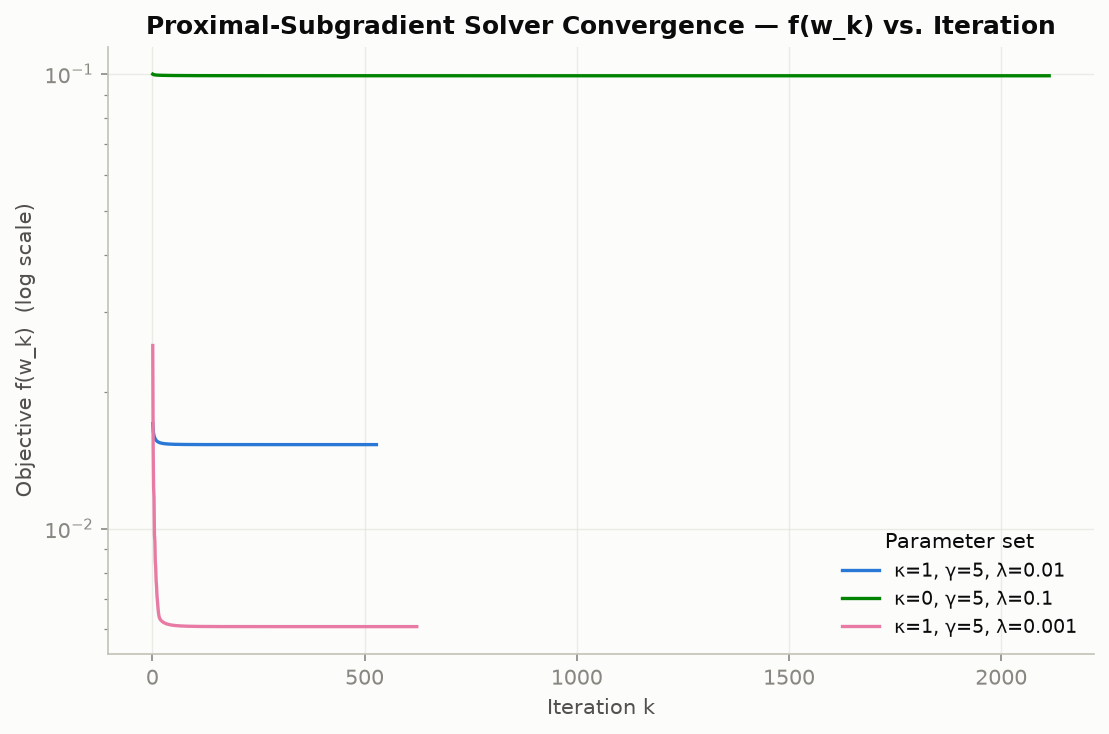
\includegraphics[width=\textwidth]{fig2_convergence.png}
    \column{0.5\textwidth}
    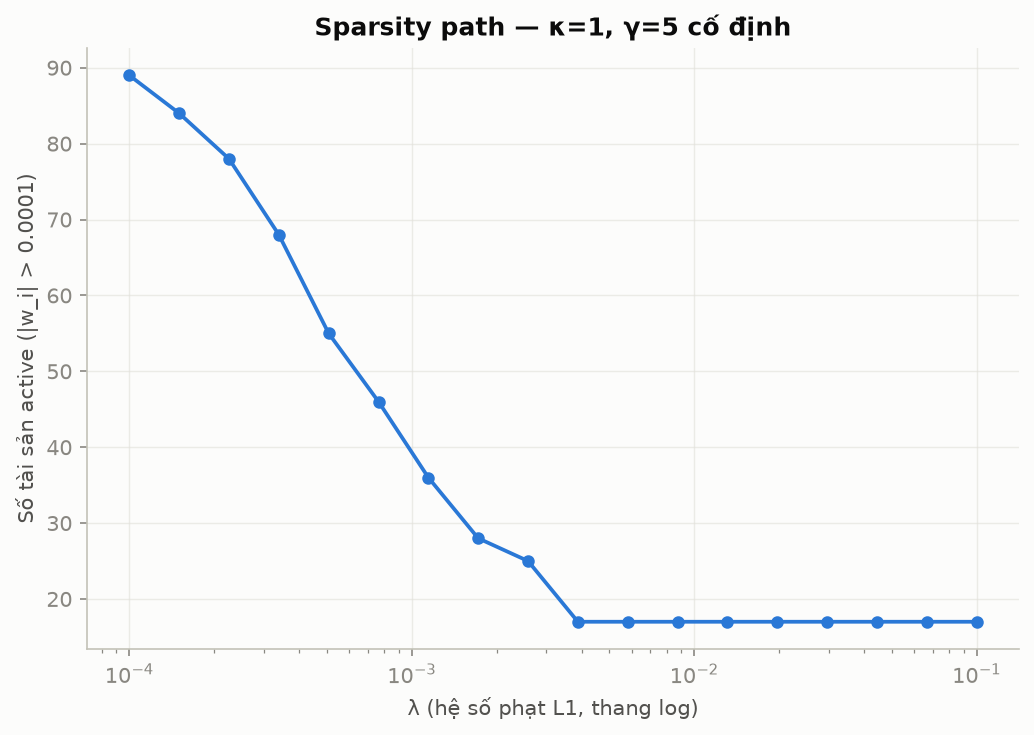
\includegraphics[width=\textwidth]{fig3_sparsity_path.png}
  \end{columns}
  \vspace{0.2cm}
  \small
  Two runs on the real 98-asset data: $(\kappa,\gamma,\lambda)=(1,5,0.01)$ converges in
  \textbf{528 iters} to \textbf{17/98} active; $(0,5,0.10)$ converges in
  \textbf{2113 iters} to \textbf{10/98} active. Zeros are \emph{exact}.
\end{frame}

\begin{frame}{A counter-intuitive finding}
  \begin{columns}
    \column{0.55\textwidth}
    Turning the robust term on ($\kappa:0\to1$) \bad{increases} concentration
    (active count \emph{and} HHI) instead of diversifying.

    \vspace{0.2cm}
    \textbf{Why:} $\kappa\norm{\Ssqrt w}_2$ is degree-1 homogeneous --- its subgradient does
    \emph{not} shrink as $\norm{w}\to0$, unlike the quadratic term. It pulls in a fixed
    direction, and with 98 heavily co-moving VN stocks, that direction favours a few names.

    \vspace{0.2cm}
    \small \textit{An empirical finding on this dataset --- not a general theorem.}
    \column{0.45\textwidth}
    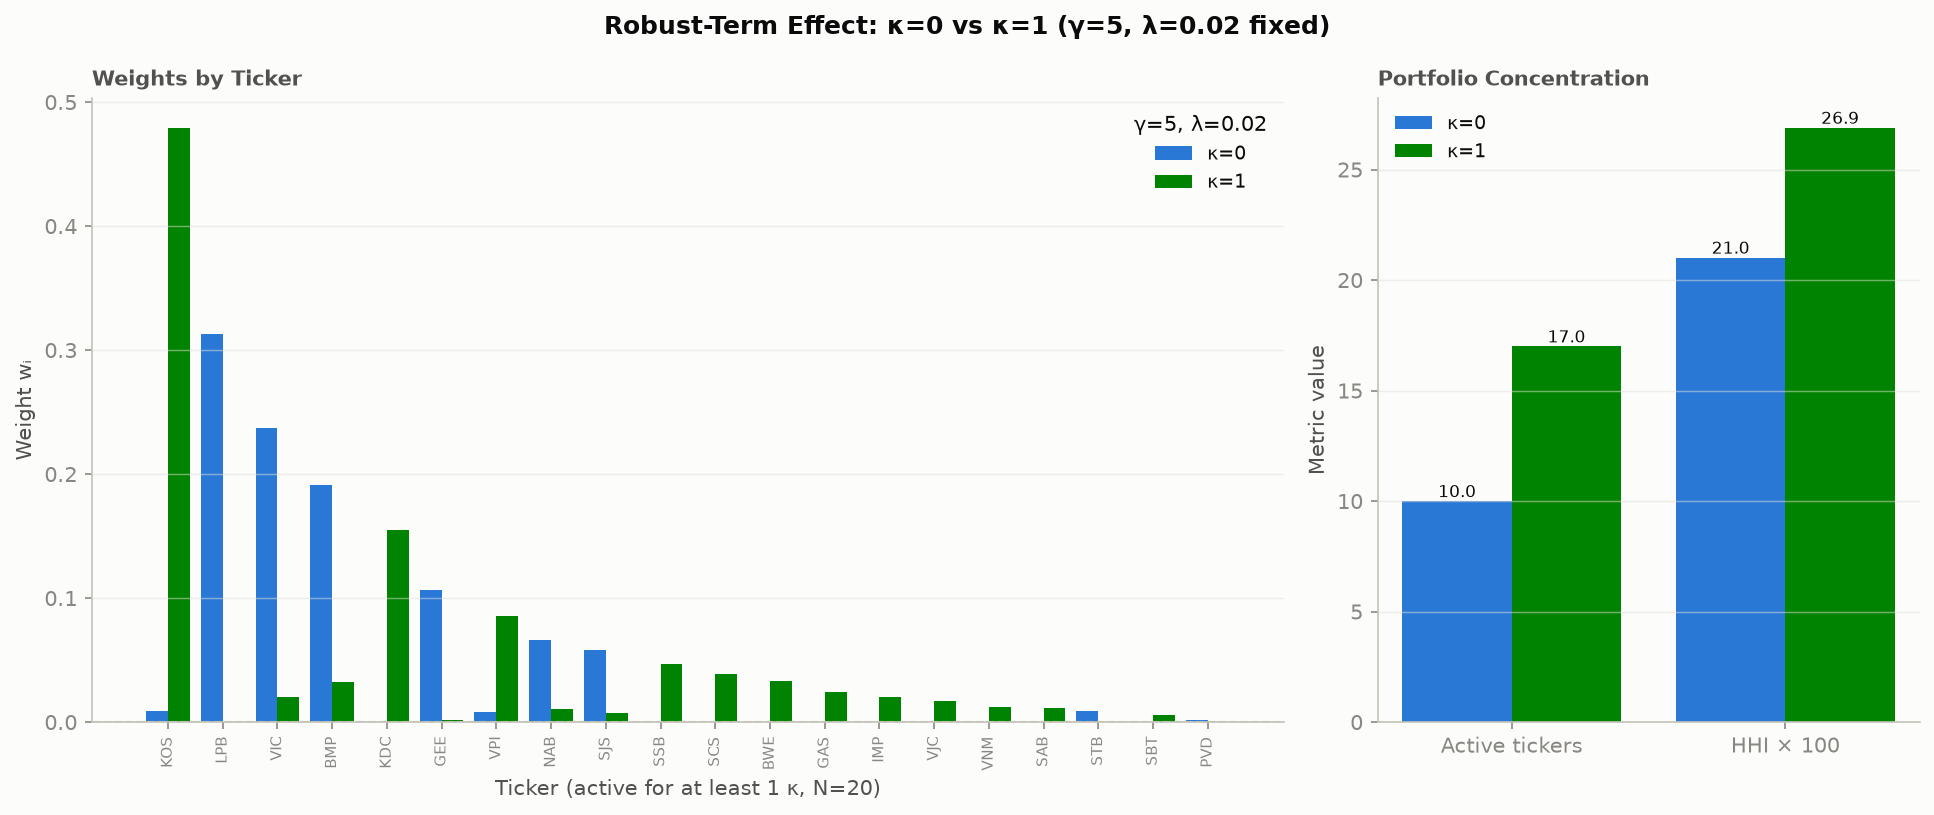
\includegraphics[width=\textwidth]{fig5_robust_effect.png}
  \end{columns}
\end{frame}

\begin{frame}{Cross-verification: hand-written vs.\ CVXPY}
  \begin{columns}
    \column{0.55\textwidth}
    \small
    \begin{tabular}{@{}rrrrr@{}}
    \toprule
    $\kappa$ & $\gamma$ & $\lambda$ & Rel.\ gap & Jaccard \\
    \midrule
    1   & 5  & 0.01  & $1.9{\times}10^{-7}$ & 1.00 \\
    0   & 5  & 0.10  & $7.8{\times}10^{-6}$ & 1.00 \\
    1   & 5  & 0.001 & $2.4{\times}10^{-7}$ & 1.00 \\
    2   & 10 & 0.05  & $-1.7{\times}10^{-8}$& 1.00 \\
    0.5 & 1  & 0.02  & $1.8{\times}10^{-6}$ & 1.00 \\
    1   & 5  & 0     & $5.1{\times}10^{-7}$ & 1.00 \\
    \bottomrule
    \end{tabular}
    \vspace{0.2cm}

    \good{Max rel.\ gap: 0.000775\%. Active set matches on 6/6.}
    \column{0.45\textwidth}
    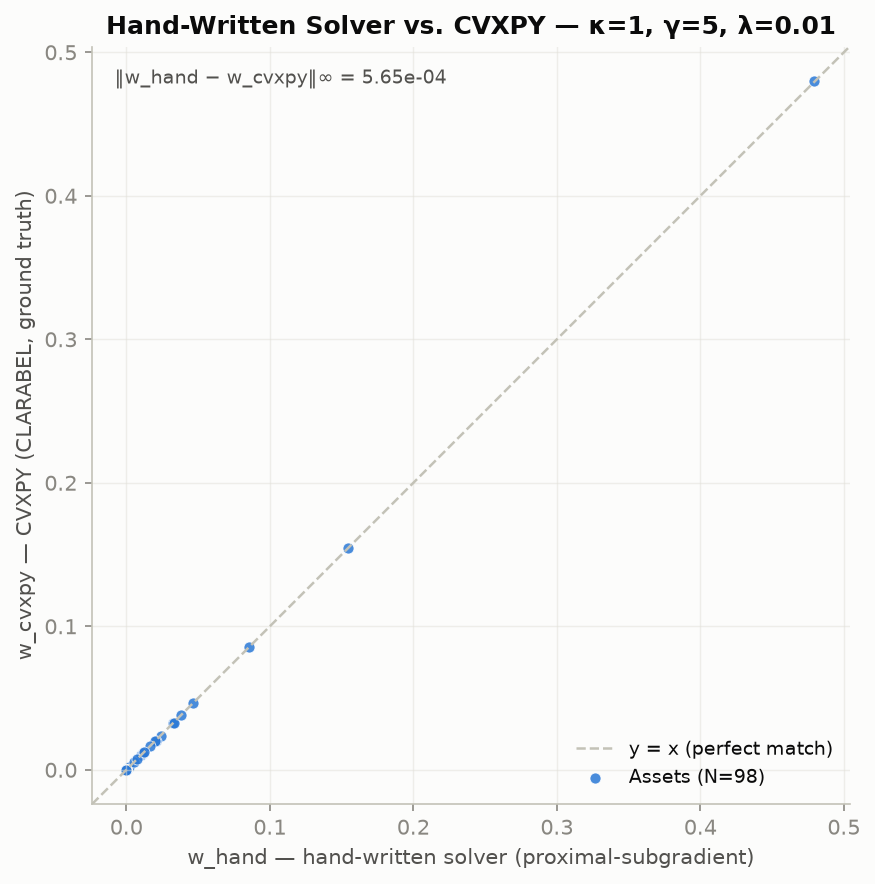
\includegraphics[width=\textwidth]{fig6_prox_vs_cvxpy.png}
  \end{columns}
\end{frame}

\begin{frame}{Walk-forward out-of-sample backtest}
  \textbf{Why:} Section~Results above optimizes on data it has already seen --- says nothing
  about deployed performance.

  \vspace{0.2cm}
  \begin{itemize}
    \item Rolling \textbf{24-month} window: 18 months fit + 6 months validate
    \item \textbf{Monthly} rebalance, \textbf{long-only} ($w\ge0$)
    \item Grid search $(\kappa,\gamma)\in\{0,0.5,1,2\}\times\{1,5,10\}$, picked by
          validation Sharpe each period
    \item Ledoit--Wolf shrinkage; \textbf{0.20\%} transaction cost per unit turnover
    \item Benchmark: \textbf{equal-weight $1/N$}, same schedule, same fees
  \end{itemize}
\end{frame}

\begin{frame}{Rolling window, concretely: three consecutive periods}
  \begin{center}
  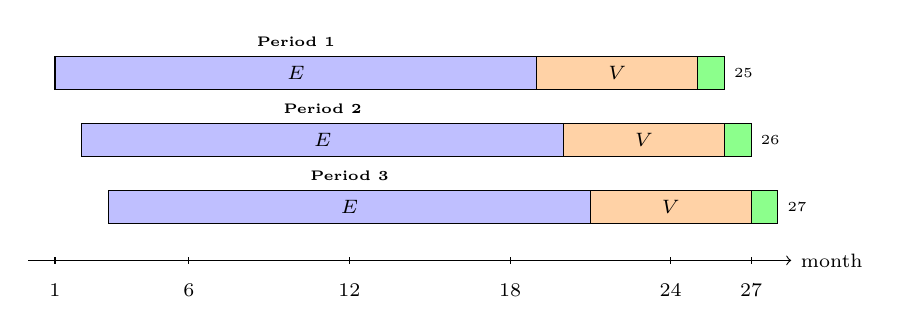
\begin{tikzpicture}[x=0.34cm, y=0.85cm, font=\scriptsize]
    % month axis
    \draw[->] (0,-0.4) -- (28.5,-0.4) node[right]{month};
    \foreach \m in {1,6,12,18,24,27} {
      \draw (\m,-0.45) -- (\m,-0.35);
      \node[below] at (\m,-0.6) {\m};
    }

    % Period 1
    \node[above,font=\tiny\bfseries] at (10,2.65) {Period 1};
    \draw[fill=blue!25] (1,2.15) rectangle (19,2.65);
    \node at (10,2.4) {$E$};
    \draw[fill=orange!35] (19,2.15) rectangle (25,2.65);
    \node at (22,2.4) {$V$};
    \draw[fill=green!45] (25,2.15) rectangle (26,2.65);
    \node[right,font=\tiny] at (26,2.4) {25};

    % Period 2 -- shifted by exactly 1 month
    \node[above,font=\tiny\bfseries] at (11,1.65) {Period 2};
    \draw[fill=blue!25] (2,1.15) rectangle (20,1.65);
    \node at (11,1.4) {$E$};
    \draw[fill=orange!35] (20,1.15) rectangle (26,1.65);
    \node at (23,1.4) {$V$};
    \draw[fill=green!45] (26,1.15) rectangle (27,1.65);
    \node[right,font=\tiny] at (27,1.4) {26};

    % Period 3 -- shifted by another month
    \node[above,font=\tiny\bfseries] at (12,0.65) {Period 3};
    \draw[fill=blue!25] (3,0.15) rectangle (21,0.65);
    \node at (12,0.4) {$E$};
    \draw[fill=orange!35] (21,0.15) rectangle (27,0.65);
    \node at (24,0.4) {$V$};
    \draw[fill=green!45] (27,0.15) rectangle (28,0.65);
    \node[right,font=\tiny] at (28,0.4) {27};
  \end{tikzpicture}
  \end{center}
  \vspace{0.1cm}
  \small
  \textcolor{blue!55!black}{\rule{0.28cm}{0.28cm}}~Estimation $E$ (18 mo) \quad
  \textcolor{orange!85!black}{\rule{0.28cm}{0.28cm}}~Validation $V$ (6 mo) \quad
  \textcolor{green!50!black}{\rule{0.28cm}{0.28cm}}~Deployed month

  \vspace{0.15cm}
  The window \textbf{slides forward by exactly 1 month} each period: Period 1 and Period 2
  share \textbf{23 of 24} months of data --- yet $(\kappa,\gamma)$ still swings between periods
  (next slides). A 6-month validation slice is a noisy yardstick even when the underlying data
  barely changes.
\end{frame}

\begin{frame}{Turnover and transaction cost --- worked example}
  At each rebalance, cost is computed from the \textbf{full} weight vector, compared against
  the \textbf{drifted} portfolio just before rebalancing --- not last period's target:
  \[
    \text{turnover} = \sum_{i=1}^{N} \bigl|w^{\text{new}}_i - w^{\text{prev, drifted}}_i\bigr|
    \qquad
    \text{cost} = \text{fee} \times \text{turnover}
  \]
  \vspace{0.15cm}
  \textbf{Example} (2 of the 98 tickers shown; every other ticker unchanged $\Rightarrow$
  contributes $0$):
  \begin{center}
  \begin{tabular}{@{}lcc@{}}
  \toprule
   & Ticker A & Ticker B \\
  \midrule
  Drifted weight, just before rebalance & 60\% & 40\% \\
  New target weight, this period        & 30\% & 70\% \\
  $|\Delta w_i|$                        & 30\% & 30\% \\
  \bottomrule
  \end{tabular}
  \end{center}
  \[
    \text{turnover} = |30\%-60\%| + |70\%-40\%| = 30\%+30\% = \good{60\%}
    \qquad
    \text{cost} = 0.20\% \times 60\% = \good{0.12\%}
  \]
  \small Deducted from the \textbf{first day's} return of the new holding period only --- the
  portfolio then drifts, untouched, for the rest of the month.
\end{frame}

\begin{frame}{Backtest results --- 494 days, 25 rebalances}
  \begin{columns}
    \column{0.48\textwidth}
    \small
    \begin{tabular}{@{}lrr@{}}
    \toprule
     & Strategy & $1/N$ \\
    \midrule
    Cumulative return & 23.9\% & 14.7\% \\
    Ann.\ volatility  & 28.7\% & 19.9\% \\
    Sharpe ($r_f{=}0$) & \good{0.524} & 0.452 \\
    Max drawdown      & \bad{$-37.9\%$} & $-20.9\%$ \\
    Total fees        & \bad{3.44\%} & 0.49\% \\
    \bottomrule
    \end{tabular}
    \column{0.52\textwidth}
    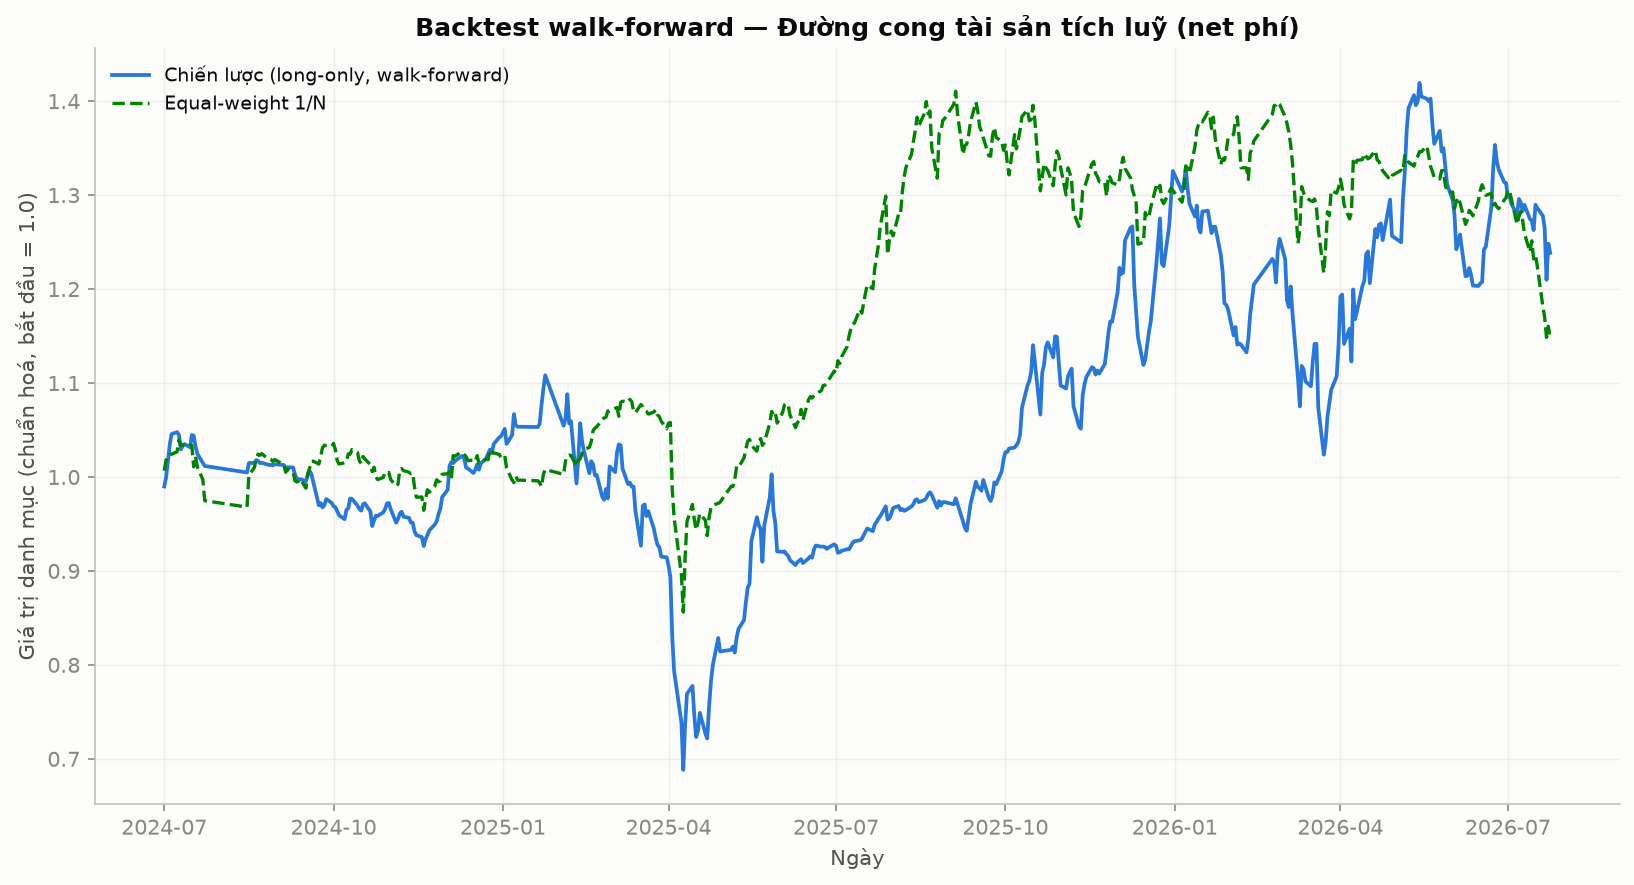
\includegraphics[width=\textwidth]{fig7_backtest_equity.png}
  \end{columns}
\end{frame}

\begin{frame}{Honest interpretation}
  \begin{itemize}
    \item<1-> \good{The win is real}: beats $1/N$ on Sharpe --- a famously hard baseline
          to beat.
    \item<2-> \bad{The win is narrow and paid for}: $\sim$44\% more volatility,
          $\sim$1.8$\times$ the drawdown.
    \item<3-> \bad{Costs are the binding problem}: $\sim$7$\times$ the fees, driven by
          $\sim$69\%/month turnover --- because $(\kappa,\gamma)$ swings between periods on a
          short, noisy 6-month validation window.
  \end{itemize}
  \onslide<4->{
  \vspace{0.3cm}
  \centering \textit{A real but modest risk-adjusted edge, not a free lunch.}
  }
\end{frame}

% ============================================================
\section{Conclusion}
% ============================================================

\begin{frame}{Limitations}
  \small
  \begin{itemize}
    \item Survivorship bias: current VN100 membership applied backward
    \item $\muhat$ remains a noisy estimator --- the robust term blunts, doesn't remove, this
    \item The $\kappa$-concentration finding is empirical, not general
    \item OOS window is short: $\sim$24 months, one market regime
    \item 6-month validation window causes mild parameter overfitting
    \item Single historical path --- no bootstrap confidence intervals
    \item Flat transaction-cost model, no slippage/market impact
  \end{itemize}
\end{frame}

\begin{frame}{Conclusion}
  \begin{itemize}
    \item Formulated a \textbf{convex, SOCP-representable} model where the robust term is
          \textbf{derived}, not assumed, and the $\ell_1$ term does double duty
          (sparsity + leverage cap).
    \item A \textbf{pure-NumPy} proximal-subgradient method, with an \textbf{exact joint prox}
          for $\ell_1$ + budget constraint, matches an independent interior-point solver to
          $7.75\times10^{-6}$ relative gap and \textbf{identical active sets}, 6/6.
    \item Out of sample: beats equal-weight $1/N$ on a risk-adjusted basis --- by a real but
          modest margin, at materially higher cost and risk.
    \item \textbf{Methodological lesson:} the prox-then-project bug was invisible to
          inspection --- found only by an independent cross-check.
  \end{itemize}
\end{frame}

\begin{frame}{References}
  \footnotesize
  \begin{itemize}
    \item H.\ Markowitz. \textit{Portfolio Selection}. J.\ Finance, 1952.
    \item S.\ Boyd, L.\ Vandenberghe. \textit{Convex Optimization}. Cambridge Univ.\ Press, 2004.
    \item N.\ Parikh, S.\ Boyd. \textit{Proximal Algorithms}. FnT Optimization, 2014.
    \item J.\ Duchi et al. \textit{Efficient Projections onto the $\ell_1$-Ball...} ICML, 2008.
    \item O.\ Ledoit, M.\ Wolf. \textit{A Well-Conditioned Estimator for Large Covariance Matrices}. JMVA, 2004.
    \item V.\ DeMiguel, L.\ Garlappi, R.\ Uppal. \textit{Optimal vs.\ Naive Diversification...} RFS, 2009.
    \item D.\ Goldfarb, G.\ Iyengar. \textit{Robust Portfolio Selection Problems}. Math.\ OR, 2003.
    \item S.\ Diamond, S.\ Boyd. \textit{CVXPY}. JMLR, 2016.
    \item Data: \texttt{vnstock} (VN100, VCI/KBS sources).
  \end{itemize}
\end{frame}

\begin{frame}
  \centering
  \Large \textbf{Thank you}
  \vspace{0.5cm}

  \normalsize Questions?
\end{frame}

\end{document}
